  \vspace{-1mm} 

This section evaluates and analyzes the performance of benchmarks for CPU, GPU, and MIC. We present the performance efficiency, energy efficiency, monetary efficiency, temperature and productivity using Nvidia K80 GPU, Intel Xeon Phi SC7120P MIC and dual Intel Xeon E5-2699 v3 CPU to evaluate performance. While CPU and MIC executables are generated from the same C source code annotated with OpenMP, GPU programs are implemented using CUDA. 


\subsection{Experimental Setup}
\bigbreak
\vspace{-4mm} 
%\noindent\textbf{Intel Xeon CPU:} 
Performance of CPU is measured with 256 GB of 2133 MHz DDR4 ECC memory, based on two-socket Intel Xeon E5-2699v3 CPUs for the server. The thermal design power (TDP) of each CPU socket is 145 W. The sockets are interconnected by a Quick Path Interconnect (QPI) link and forming a shared-memory NUMA system. Each socket has 18 physical cores (36 cores in the system) clocked at 2.3 GHz (turbo frequency of 3.6 GHz) with two-way hyper-threading. The vector units of the system support the AVX instruction set with 256-bit vector registers. The host operating system is CentOS 6.7 Linux with kernel version 2.6.32-573.12.1.el6.x86\_64. The code was compiled with the Intel icc compiler version 13.1.3.

\vspace{-4mm}

% Table generated by Excel2LaTeX from sheet 'Sheet1'
\begin{table}[htbp]
  \centering
      \caption{Complete System Specification}
    \begin{adjustbox}{width=0.5\textwidth}
    \begin{tabular}{rccc}
    \toprule
          & GPU   & MIC   & CPU x 2 \\
    \midrule
    Model & Tesla GK210 & Xeon Phi SC7120P & Xeon E5-2699 v3 \\
    Core  & 2496  & 61    & 36 \\
    Core Clock (GHz) & 0.56  & 1.24  & 2.3 \\
    SP TFLOPS & 4.37  & 3.11  & 1.3 \\
    DP TFLOPS & 1.45  & 1.55  & 0.65 \\
    Memory Size (GB) & 24    & 16    & - \\
    Mem. Bandwidth(GB/s) & 240   & 352   & 136 \\
    Monetary Cost (USD) & 2499  & 3749  & 9800 \\
    Max Power Usage (TDP) & 150   & 300   & 290 \\
    \bottomrule
    \end{tabular}%
    \label{tab:specification}
    \end{adjustbox}

\end{table}%

\vspace{-1mm}

 GPU is measured in the same system as CPU. The GPU model used for the results presented in this paper is the Nvidia Tesla K80 (active-cooled model for workstations), which has two Tesla GK210 GPUs. Characteristics for both GPUs are 2496 cores clocked at 560 MHz, 24 GB of on-board memory with a clock of 2.5 GHz, and a 384-bit memory interface. The code was written in CUDA and C compiled with the nvcc compiler, version 7.5. 


%\noindent\textbf{Intel Xeon Phi Coprocessor:} 
With regard to Intel MIC, it is measured in the same system and Intel icc compiler as CPU. The system contains one MIC coprocessor, Xeon Phi QS-7120P (passive-cooled model for servers) with 61 cores at 1.24 GHz, C0 coprocessor stepping, and 16 GB of GDDR5 RAM at 2.75 GHz. The driver stack is MPSS, version 2.1.6720-13. 



\subsection{Performance and Performance Efficiency\\}
\vspace{-4mm} 
Performance and efficiency are two most important factors to evaluate architectures of CPU, GPU and MIC. Execution time can be utilized as performance. However, since CPU, GPU and MIC are implemented in different architectures and they are designed in diverse hardware cores that have different definition and standard, it’s hard to compare performance efficiency between different architectures. One way to compare their performance is the peak floating-point operations per second (FLOPS). In order to get fair results, we choose problem size of benchmarks that are large enough to eliminate the influence of instant change of performance, power consumption, temperature and data transfer in and out of GPU/MIC. Problem sizes of all applications are fixed at 12000 for LUD, 193000 for CFD, 32000 for NW, 64M for BFS and 1024 with 20000 loops for Hotspot. Threads available are assigned in maximum for CPU, GPU and MIC. The execution time shown is an average over ten runs.

The performance are summarized as speedup in Fig. \ref{fig:speedup}. It presents the average normalized execution time observed for LUD, CFD, NW, BFS and HotSpot. The result shows the speedup of each application running on a K80 GPU and a SC7120P MIC relative to a dual Intel Xeon E5-2699v3 CPU. The speedups of GPU range from 2.3-103X as CPU implementations and the speedups of MIC range from 1.2-24X as CPU implementations excluding BFS.
  
With respect to GPU and MIC, data is copied to and from the accelerator/coprocessor under the explicit control from the programmer and runtime. Programmers mark code blocks with C/C++ pragmas for MIC and leverage runtime library for GPU. The compiler runtime transfers data from the host to the device, performs computation on the device and returns results back to the host. From Fig. \ref{fig:speedup}, GPU outperforms MIC by 2 to 33 times. GPU is better than MIC at handling huge data because of its streaming multi-processor (SM) that can handle millions of threads.  

The stream mechanism offered by CUDA allows the hiding of the communication overhead, in particular of the copies between CPU and GPU, provided that the computation executed concurrently with the communication is large enough. MIC is incapable of overcoming the extra processing capabilities even though MIC has superior memory transfer latency. The overheads of MIC, e.g., data offloading overheads of memory transfer and computation overheads between CPU and MIC, are much more than GPU in the benchmarks. In native mode of MIC, application directly executes on coprocessor without being offloaded to coprocessor. Such applications are required to be compiled and built on the host system using -mmic supporting flag which enables the compiler to generate an object file for Xeon Phi architecture. Executing applications in native mode requires all the dynamic libraries and executable must be present on coprocessor. MIC can take advantage of the native mode and would outperform GPU. But with respect to the benchmarks, the implementation for MIC is offload mode instead of native mode. Running on an MIC in offload mode is possible to emulate the CUDA streaming mechanism that supports independent execution flows. The performance of an MIC remains low in offload mode compared to a GPU with the same number of computing unit for a problem of fixed size. 

\vspace{-1mm}

    \begin{figure}[h!]
  \centering
  \begin{minipage}{0.5\textwidth}
    \centering
   \centering
     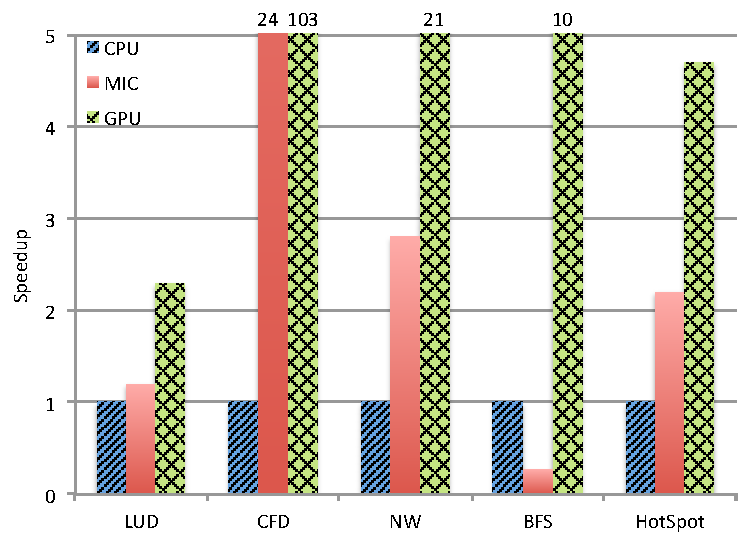
\includegraphics[width=1\linewidth]{Speedup.pdf}    
\caption{Performance comparison among CPU, GPU and MIC on speedup is normalized against CPU for LUD, CFD, NW, BFS and HotSpot. Each value is the average of ten runs. GPU outperforms CPU and MIC for execution time performance.}

\label{fig:speedup}
\end{minipage}%
\end{figure}

\vspace{-1mm}
  
  For traditional homogeneous architectures, the performance efficiency is defined as follows. Let $T_{s}$ represent execution time for serial computing of one core, $P$ is the number of cores and $T_{p}$ is the execution time for concurrent computing with the number of $P$ cores in a given application. Thus the speedup $S_{p}$ and performance efficiency $E_{p}$ are defined as:
\vspace{-1mm} 
\begin{equation}\label{equ:old_speedup}
	{S_{p}} = \frac{T_{s}}{T_{p}} \quad and \quad {E_{p}} = \frac{S_{p}}{P}
\end{equation}
  
 Since the benchmarks are designed using single precision floating point for computation, the theoretical peak FLOPS of CPU, GPU and MIC in this system are respectively 1.3 TFLOPS (Tera FLOPS), 3.11 TFLOPS and 4.87 TFLOPS. We use CPU as the baseline and normalize the performance efficiency. Let $T_{b}$ denote base execution time and $T_{t}$ denote target execution time. $S_{p}$ represents speedup calculated as the ratio of $T_{b}$ to $T_{t}$. The theoretical peak FLOPS performance of heterogeneous architectures is denoted as $F_{t}$. Thus the formula of performance efficiency $E_{p}$ is as follows:

\vspace{-1mm} 
\begin{equation}\label{equ:new_speedup}
	{S_{p}} = \frac{T_{b}}{T_{t}} \quad and \quad {E_{p}} = \frac{S_{p}}{F_{t}}
\end{equation}
  
Performance efficiency represents the gap between practical performance and theoretical performance in heterogeneous architectures, which is a critical consideration to find out the factors to improve architecture designs. From Fig. \ref{fig:performanceE}, we conclude that CPU has a better performance efficiency than GPU in LUD and better than MIC in LUD, BFS and HotSpot. Since the theoretical performance of GPU is 3.4X as CPU, but the practical speedup is only 2.3X as CPU, the performance efficiency of CPU is better than GPU in LUD. With respect to MIC, similarly even though MIC has 1.2X and 2.2X better practical performance than MIC in LUD and HotSpot respectively, MIC has 2.4X better theoretical performance than CPU. Therefore, the performance efficiency of CPU is better than MIC in LUD and HotSpot.

\vspace{-1mm}

    \begin{figure}[h!]
  \centering
  \begin{minipage}{0.5\textwidth}
    \centering
   \centering
     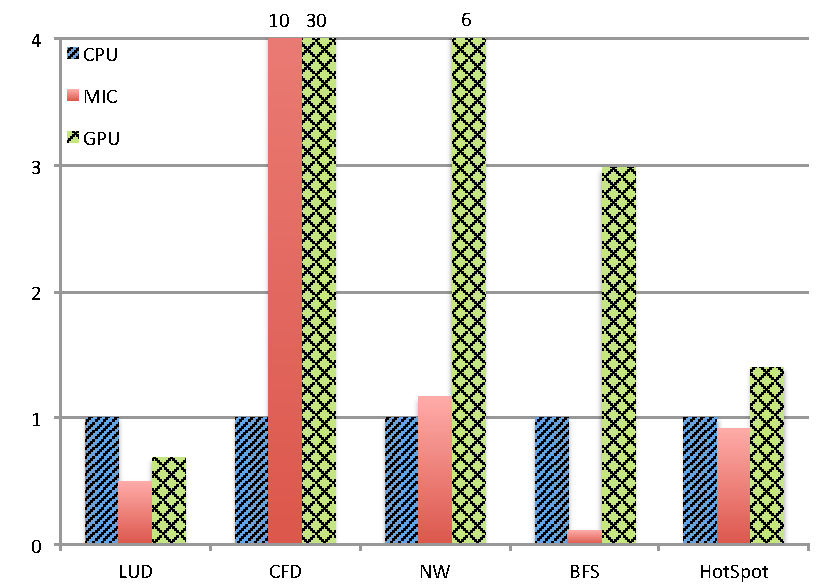
\includegraphics[width=1\linewidth]{Performance_E.pdf}  

\caption{Performance efficiency is based on practical performance and theoretical performance. The comparison among CPU, GPU and MIC uses CPU execution time as baseline for LUD, CFD, NW, BFS and HotSpot.}
\label{fig:performanceE}
\end{minipage}%
\end{figure}

\vspace{-1mm}

    
New challenges need to be solved in order to analyze monetary cost corresponding to the performance of GPU, MIC and CPU especially in computing centers where makes an efficient or suitable decision balancing the performance and cost. Thus the monetary cost efficiency is important to consider. Let $S_{p}$ and $C$ represent speedup of performance and monetary cost, respectively. We utilize CPU as the baseline and normalize the performance efficiency so the formula of monetary cost efficiency $E_{c}$ is as follows:
\vspace{-1mm} 
\begin{equation}\label{equ:monetaryE}
	{E_{c}} = \frac{S_{p}}{C}
\end{equation}
  

  \vspace{-2mm} 
  
\subsection{Power Consumption and Energy Efficiency\\}
\vspace{-4mm} 

There are growing numbers of commercial high performance computing solutions using various accelerators. Therefore, power consumption has increasingly become a concern. In addition, a better understanding of the power tradeoffs of heterogeneous architectures is needed to guide usage in server clusters and data centers. 

NVML (Nvidia Management Library) \cite{R:16} is a runtime library to measure power consumption when executing the kernel. However, since nvidia-smi is a high-level interface allowing administrators to query GPU information in command line, the rate of sampling power consumption is very low so that we could not record the change in power until the kernel is running for a very long time. The nvmlDeviceGetPowerUsage function in the NVML library obtains the power consumption  for GPU in milliwatts. The power consumption is obtained for the entire board. The power consumption is accurate within +/- 5 watts error with precision in milliwatt and is updated at roughly 60Hz. To measure the runtime power of a kernel with the NVML library for lowest overhead, we run NVML on a thread and the kernel on other threads. We choose Pthread because it reduces overhead, and the only communication we would like to have with the main thread is a flag variable and a variable to store power readings which is set to be volatile. The thread running NVML stops when the flag is reset, which is when the GPU kernel stops executing. The temperature is provided by integrated sensors inside the device.

 Power consumption of MIC is calculated by the approximation of power timeslices provided by MIC System Management Control (micsmc) \cite{R:17} which has direct connection to the coprocessor I2C interface \cite{R:18}, an on-board I2C sensor bus and a third interface through the SMBus pins of the PCI Express connector to the system management solution which is used for obtaining data including frequency, power, temperature, memory usage, and CPU utilization per core. However, as additional types of data are requested, the delay between calls increase. Therefore, to capture the energy readings in the smallest timeslice available, only temperature and power data are recorded (both are printed when the same input parameter is given). The micsmc tool measures and reports every 22–28ms, which is sufficient for a detailed evaluation. 

 Recent Intel SandyBridge chips include the “Running Average Power Limit” (RAPL) interface \cite{R:15} which is designed to provide an infrastructure for keeping processors inside of a given user-specified power envelope. RAPL supports power capping PKG, PP0 and DRAM power planes by writing into the relevant model specific register (MSR). The internal circuitry can estimate current energy usage based on a model driven by hardware counters and temperature. The results of this model are available to the user via a MSR which can be accessed to get power consumption for each power plane with an update frequency on the order of milliseconds. 

 Idle power is the power consumed by the devices when the device is in a long idle state, i.e., when the devices are doing nothing for a long period of time. As Fig. \ref{fig:power} illustrates, at the idle state the power consumption of CPU is much lower than GPU and MIC and is evaluated 28\% and 19\% for GPU and MIC respectively. With respect to the benchmarks, MIC consumes more power than GPU except HotSpot and CPU except NW. The power consumption of MIC is 1.01-2.37X as GPU and 1.20-1.68X as CPU. GPU consumes more power than MIC and CPU in HotSpot while CPU consumes more power than MIC and GPU in NW. One reason is that certain factors of power consumption of MIC such as the execution of the graphics pipeline, bus communication and memory access consume more power than the corresponding parts of GPU. For certain benchmarks, GPU and MIC are more effective than CPU for the computations that use a small size of input data in communication between the host and devices and perform well in compute-intensive operations which reduce the workload of communication and computation to decrease power consumption. For some workload, memory-bound causes a decrease in power consumption, as the duration of execution is reducing, consuming less cumulative power. In other words, intensive workload of MIC and GPU should generally use the high core clock so that it completes operation as soon as possible to minimize energy. 
 %The reason might be that NW and HotSpot take more memory accesses than LUD, CFD and BFS, and that MIC uses less energy for memory accesses.

    \begin{figure}[h!]
  \centering
  \begin{minipage}{0.5\textwidth}
    \centering
   \centering
     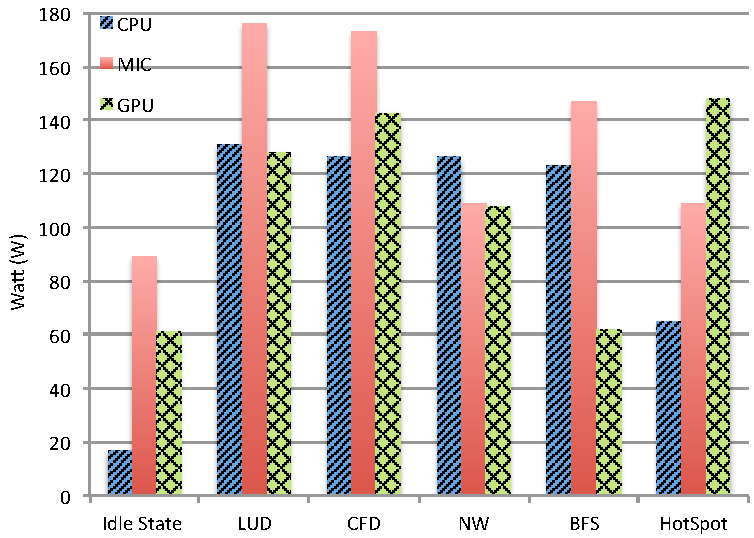
\includegraphics[width=1\linewidth]{Power.pdf}    
\caption{Power consumption comparison among CPU, GPU and MIC for idle state, LUD, CFD, NW, BFS and HotSpot.}
\label{fig:power}
\end{minipage}%
\end{figure}

\vspace{-2mm}

With regard to scientific computing programs, FLOPS per watt has gained popularity in evaluating energy efficiency of high performance computing applications. Practical FLOPS and power consumption are respectively denoted as $F_{p}$ and $P$. We utilize CPU as the baseline and normalize the energy efficiency so the formula of energy efficiency $E_{e}$ is as follows:
\vspace{-1mm} 
\begin{equation}\label{equ:energyE}
	{E_{e}} = \frac{F_{p}}{P}
\end{equation}
  
According to our measurement in Fig. \ref{fig:energyE}, GPU outperforms MIC and CPU in all benchmarks while MIC outperforms CPU in CFD, NW and HotSpot. Because FLOPS of GPU in the benchmarks is higher than MIC and CPU, even though the power consumption of GPU is more than MIC and CPU in HotSpot, GPU still has better energy efficiency. With respect to LUD between MIC and CPU, because the power consumption of MIC in LUD is 1.4X as CPU and MIC performs 1.2X better FLOPS performance than CPU, CPU outperforms MIC.

  \vspace{-2mm} 
    \begin{figure}[h!]
  \centering
  \begin{minipage}{0.5\textwidth}
    \centering
   \centering
     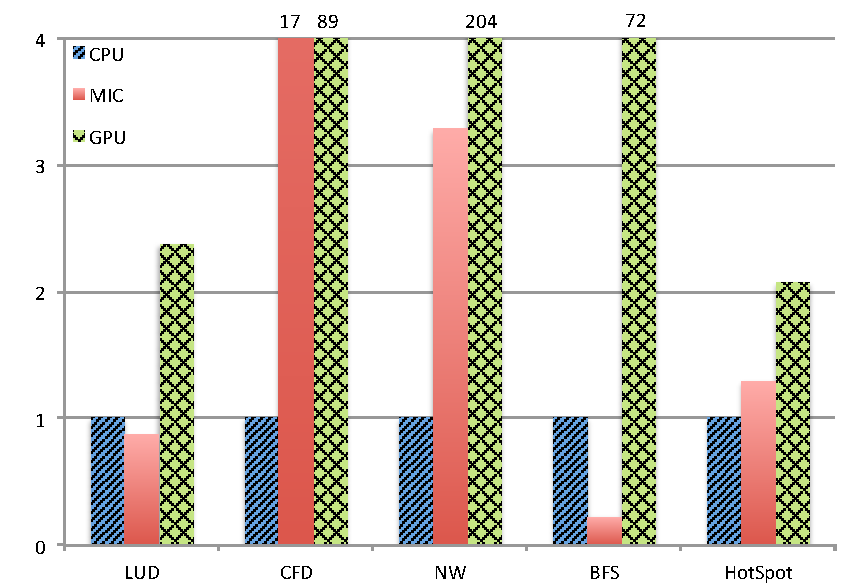
\includegraphics[width=1\linewidth]{Energy_E.pdf}    
\caption{Energy efficiency is the efficiency of the practical FLOPS to power consumption on devices of heterogeneous architectures for each benchmark using CPU as baseline. GPU performs better than CPU and MIC for five benchmarks on energy efficiency.} 
\label{fig:energyE}
\end{minipage}%
\end{figure}

  \vspace{-2mm} 
\subsection{Temperature\\}
\vspace{-4mm} 

Temperature of running kernels on heterogeneous architecture devices is also a critical consideration for high performance computing in server clusters and data centers because we need to pay for cooling down systems and to utilize them efficiently. 

By comparing results in Fig. \ref{fig:temperature}, MIC stays in higher temperature than GPU and CPU, and GPU stays in higher temperature than CPU. In addition, we observe that for MIC and GPU even though the temperature of GPU is only 80\% of MIC in HotSpot, power consumption of GPU is 1.4X as MIC, which means that for some benchmarks even though GPU consumes more power for calculation than MIC, MIC stays in higher temperature than GPU. With regard to other benchmarks, the power consumption of MIC is 1.01-2.37X as GPU which the temperature is 1.04-1.25X as GPU. From Fig. \ref{fig:temperature}, CPU performs lower than MIC and GPU especially in idle state. The temperature of CPU is 63-83\% of MIC for benchmarks and 59\% in idle state while CPU is 77-100\% of GPU excluding HotSpot and 63\% in idle state. Because the design for CPU is for general purpose and task scheduling in the whole system, the temperature of CPU must stay low in idle for some applications using less intensive computing. But the purpose of MIC and GPU is for high throughput and intensive computing, which in architecture design is one of the reasons why temperature of MIC and GPU is higher than CPU.

    \begin{figure}[h!]
  \centering
  \begin{minipage}{0.5\textwidth}
    \centering
   \centering
     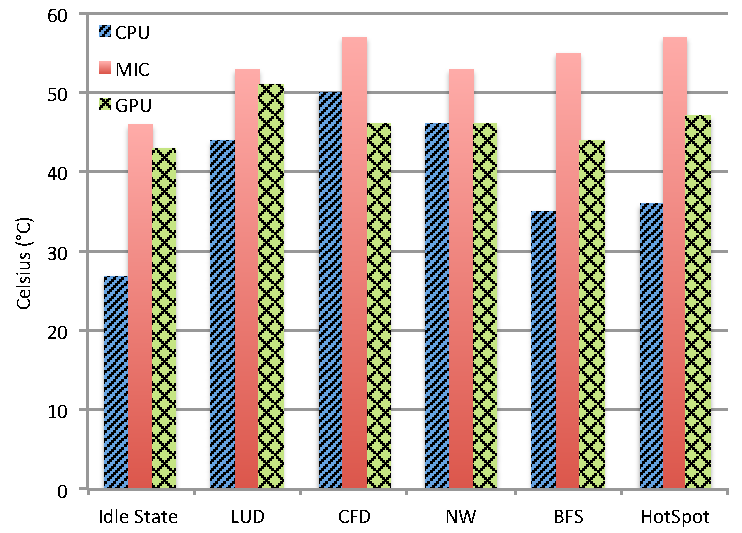
\includegraphics[width=1\linewidth]{Temperature.pdf}    
\caption{Temperature comparison among CPU, GPU and MIC for idle state, LUD, CFD, NW, BFS and HotSpot.}
\label{fig:temperature}
\end{minipage}%
\end{figure}

\subsection{Monetary Cost Efficiency\\} 
\vspace{-4mm} 
Monetary cost efficiency represents the efficiency of the performance speedup to monetary cost paid for heterogeneous architectures on specific mainstream CPU, GPU and MIC, which also refers to the performance speedup of heterogeneous architectures per dollar. The monetary cost is presented in Table \ref{tab:specification}. From Fig. \ref{fig:monetaryE}, the monetary cost efficiency of GPU performs well than CPU and MIC for the benchmarks because the monetary cost of CPU is 3.9X as GPU and the monetary cost of MIC is 1.5X as GPU. With regard to CPU and MIC, the monetary cost efficiency of MIC is better than CPU for the benchmarks excluding BFS because the speedup performance of CPU is 3.3X as MIC but the monetary cost of CPU is only 2.6X as MIC. Since the speedup performance of MIC in BFS is only 30\% of CPU, the monetary cost efficiency of CPU is still better than MIC in BFS.

    \begin{figure}[h!]
  \centering
  \begin{minipage}{0.5\textwidth}
    \centering
   \centering
     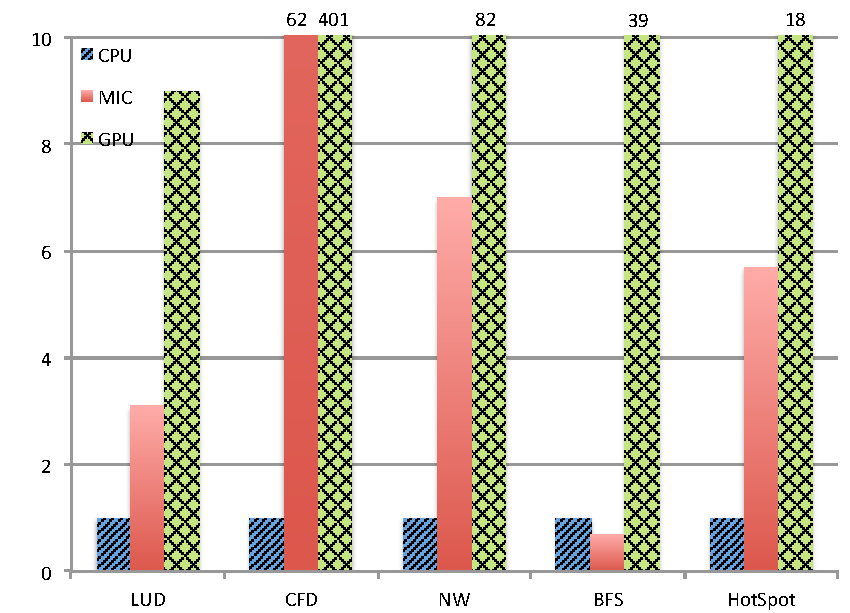
\includegraphics[width=1\linewidth]{Monetary_E.pdf}    
\caption{Monetary cost efficiency is the efficiency of the performance speedup using CPU as baseline to monetary cost paid for devices of heterogeneous architectures. GPU performs better than CPU and MIC for five benchmarks on monetary cost efficiency.}
\label{fig:monetaryE}
\end{minipage}%
\end{figure}


\subsection{Productivity of Programming\\} 
  \vspace{-4mm} 
As we know, the productivity of programming is difficult to measure under a standard approach because the ability of each programmer and the characteristics of each programming language is totally different. One way to compare the productivity of programming for different language is the source lines of code (SLOC). SLOC is one of the most widely used sizing metric in industry and literature. It is the key input for most of major cost estimation models such as COCOMO, SLIM, and SEER-SEM.  Its long-standing tradition is due to the fact that SLOC is the direct result of programming work as the most perceivable indicator of software cost. The SLOC counting standard \cite{nguyen2007sloc} is followed for all SLOC measurements for applications of heterogeneous architectures.

 The advantage of the programming models for MICs and CPUs is reducing source code size. In principle, one of the main advantages of the Intel MIC technology, with respect to other coprocessors and accelerators, is the simplicity of the porting. Programmers compile their existing source codes specifying MIC as the target architecture. Classical programming languages used in high performance computing – Fortran/C/C++ – as well as well known parallel paradigms – OpenMP or MPI – may be directly employed regarding MIC as a “classic” x86 based (many-core) architecture. An Intel MIC may be accessed directly as a stand-alone system running executables in the native mode. However, offload execution mode is available and used more widely. Adopting the offload execution model, a code runs mostly on the host but selected regions of the code are marked through directives or APIs to be executed on MIC coprocessor. On the contrary, the porting from the classical programming languages such as Fortran/C/C++ to CUDA needs more effort because CUDA is a significantly different programming model.

  
    \begin{figure}[h!]
  \centering
  \begin{minipage}{0.5\textwidth}
    \centering
   \centering
     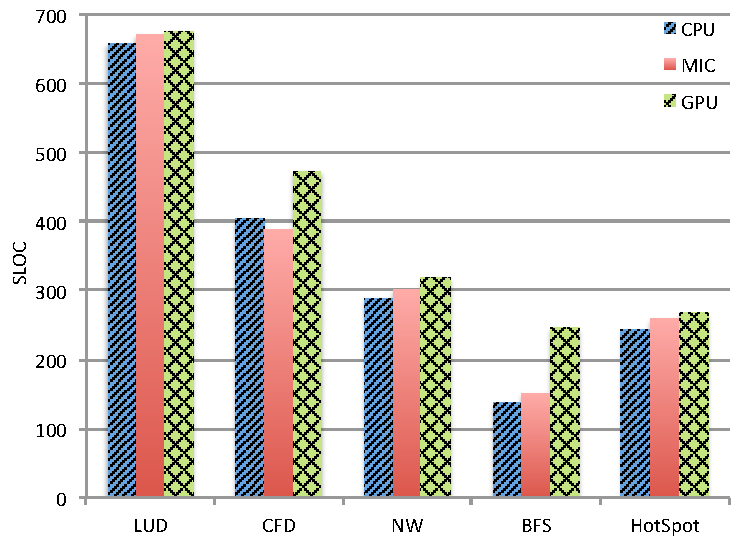
\includegraphics[width=1\linewidth]{SLOC.pdf}    
  \caption{SLOC comparison among CPU, GPU and MIC for LUD, CFD, NW, BFS and HotSpot.}
  \label{fig:sloc}
\end{minipage}%
\end{figure}

    \vspace{-2mm} 
\subsection{Unified Efficiency Metric\\}
\vspace{-4mm} 

To gain further insights into the performance of each benchmark, this work considers a unified efficiency metrics  obtained from performance efficiency, energy efficiency and monetary efficiency for overall comparison of the three architectures. The main idea of the unified efficiency metric is that different efficiency represents the strengths and weaknesses of different architectures.
\vspace{-1mm}

    \begin{figure}[h!]
  \centering
  \begin{minipage}{0.5\textwidth}
    \centering
   \centering
     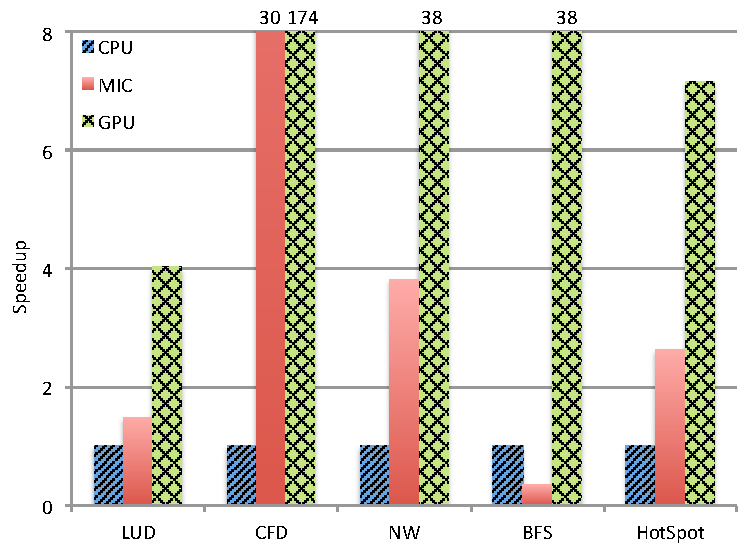
\includegraphics[width=1\linewidth]{Metric.pdf}    
  \caption{Unified efficiency metric leverages performance efficiency, energy efficiency and monetary efficiency comparing strengths and weaknesses of CPU, GPU and MIC.}
  \label{fig:metric}
\end{minipage}%
\end{figure}

\vspace{-1mm}

Let $E_{p}$ represent performance efficiency that is the ratio of speedup (based on CPU) to the theoretical peak performance of the target, $E_{e}$ be the energy efficiency that is the ratio of practical FLOPS to average power consumption of the specific application for different target devices, and $E_{c}$ represent monetary cost efficiency that is the ratio of speedup to monetary cost. Let $S_{p}$ represent speedup; $F_{t}$ represents theoretical peak FLOPS; $F_{p}$ represents practical FLOPS; $P$ represents power consumption; and $C$ represents monetary cost. The unified efficiency metric $E_{u}$ formula is as follows:
\vspace{-1mm} 
  \begin{equation}\label{equ:metric1}
    \begin{split}
  {E_{u}} &  = E_{p}+E_{e}+E_{c} \\
   & = \frac{S_{p}}{F_{t}}+\frac{F_{p}}{P}+\frac{S_{p}}{C}
  \end{split}
\end{equation}
  
Let $T_{b}$ denote base execution time, $T_{t}$ denote target execution time and $F_{a}$ denote the number of floating-point operations. Since $S_{p}$ = $T_{b}$ / $T_{t}$ and $F_{p}$ = $F_{n}$ / $T_{t}$, the metric $E_{u}$ is as follows:
  \vspace{-1mm} 
  \begin{equation}\label{equ:metric1}
    \begin{split}
  {E_{u}} &  = \frac{S_{p}}{F_{t}}+\frac{F_{n}}{P*T_{t}}+\frac{S_{p}}{C} \\
   & = {S_{p}}(\frac{1}{F_{t}}+\frac{F_{n}}{P*T_{b}}+\frac{1}{C})
  \end{split}
\end{equation}

  
 From Fig. \ref{fig:metric}, GPU is still better than MIC and much better than CPU for the benchmarks. This illustrates that when combining performance efficiency, energy efficiency and monetary cost efficiency, GPU performs better compared to CPU and MIC for the benchmarks. Since MIC outperforms CPU for the benchmarks excluding BFS, for some intensive computing applications designed for HPC in heterogeneous computing infrastructures such as BFS, CPU still outperforms MIC when we consider overall benefits.